\documentclass{thesis}

% TX Fonts を使う
\usepackage{txfonts}
\usepackage{url}
\usepackage{algorithm}
\usepackage{algorithmic}
\usepackage[dvipdfmx]{color}
\usepackage{multirow}
\usepackage{subfigure}
\usepackage{indentfirst}

\begin{document}

% 目次
\tableofcontents
%--ここから本文---
\chapter{序論}
%第1章 まえがき

%1章1節
\section{研究背景および目的・目標}
近年では,IoT(Internet of Things)の普及が進んでおり,様々なものがインターネットに繋がる時代である.インターネトに繋がるものをIoT機器(IoTデバイス)といい,例として家電や自動車・産業用ロボットなどが挙げられる.
IoTを実現する上で,周囲の情報を検知するセンシングデバイスやネットワークは必要不可欠である.
そして,センシングデバイスがインターネットに繋がることで,外部の悪意のある第三者からの攻撃により,データを盗聴・改ざんする恐れが懸念される.

第三者からの攻撃事例に,タイヤ空気圧監視システムへの攻撃事例がある\cite{maegaki}.
タイヤ空気圧監視システム(TPMS:(Tire Pressure Monitoring System))とは,
タイヤの空気圧を常時監視するシステムであり,空気圧が低いタイヤで高速走行をすることによるタイヤバースト事故を防ぐ効果が期待される.
しかし,このTPMSの無線通信には脆弱性があることが問題となっている.
その問題の一つとして,TPMSでは通信メッセージが暗号化されていないため,盗聴解析が容易になるという点がある.
また, TPMSの空気圧報告メッセージになりすますことができるという問題点もある.
この事例から,センシングデバイスにおいて,ネットワーク上の脆弱性があることで外部からの攻撃によるデータの盗聴・改ざんが行われてしまうリスクがあることから,セキュリティ対策が不可欠となることが分かる.

センシングデバイスのセキュリティ対策の一つに認証・暗号化がある.
しかしながら,AESなど従来の暗号化方式は処理負荷が高いことから処理性能の低いセンシングデバイスには導入困難であるため,現在市場に出回っているセンシングデバイスには認証・暗号化といったセキュリティ対策が不十分で,脆弱性があると考えられる.
そこで,センシングデバイスなど,処理性能の低いIoT機器において,
極めて小さい処理負荷で認証と暗号化通信のできる軽量なセキュリティ対策が求められる.

本研究では,処理能力の低いセンシングデバイスで構成されるIoTシステムにおいて,デバイスとエッジサーバー間の
安全なデータ通信を行うセキュアな組込みシステムを開発することを目的とする.
具体的には,高知工学科大学の清水明宏教授が処理能力の低い装置へのセキュリティ機能実装のために
開発されたワンタイムパスワード認証方式SAS-L2をIoTセンシングデバイス
に実装することで,デバイス間の相互認証およびセンシングデータの暗号化通信方法を実現する.
なお,本研究は,2人チーム(浅野美咲,内山田隆太)でV字開発モデルに従って処理能力の低いセンシングデバイスで構成されるSAS-L2認証を導入したセキュアなIoTシステムの開発を行う.
システムの設計にはUMLを利用する.
チームメンバーの2人で分担し,内山田がエッジサーバーの実装,浅野がエッジデバイスの実装を行う.




%1章2節

\section{本論文の構成}
本論文の構成は以下の通りである.
第1章では,研究の背景および目的・目標について述べる.
第2章では,本論文に必要な暗号化手法と通信プロトコル,システム開発プロセスに関する用語について述べる.
第3章では,SAS-L2認証について述べる.
第4章では,センシングデータ通信の暗号化について述べる.
第5章では,開発したシステムの概要について述べる.
第6章では,システムの設計・テスト項目について述べる.
第7章では,実装したシステムの検証結果と考察を述べる.
第8章では,本論文のまとめを述べる.


\chapter{準備}
%第2章:準備
 本章では、システム開発の進め方と、設計の工程で作成したUML図について説明する。

\subsection*{V字モデル\cite{kumikomi}}
ソフトウェアを開発する上では、適切な開発プロセスに沿って作業を進める必要がある。本研究では、開発プロセスのモデルの一つであるV字モデルを採用し、開発を進めた。このモデルを用いた場合の、各プロセスの進め方を図\ref{buiji}に示す。このモデルではテストを重視しており、図\ref{buiji}からもわかるように、左側にある分析や設計、実装のプロセスと、各テストの工程との対応が理解しやすく、検証の段階において、検証の対象とすべき範囲が把握しやすいという利点がある。例えば、要求分析に対してはシステムテストが配置され、実装に対しては単体テストが配置されている。これは、プログラム作成などの実装の正しさを単体テストによって確認し、要求分析の正しさをシステムテストで確認することを示している。そして右側のテストの各プロセスで不具合が見つかった場合には、左側の対応するプロセスに戻って修正を行うことになる。本研究でも、このような開発プロセスモデルの手順に沿い、必要に応じて、前のプロセスに立ち返りながら、運用に至るまでのプロセスを進めた。なお、本論文ではシステムテストと同じ意味を持つ言葉として、総合テストという言葉を用いている。

\begin{figure}[htbp]
	\centering
	\includegraphics[width=12cm]{buiji.eps}
	\caption{V字モデル}
	\label{buiji}
\end{figure}


\subsection*{UML\cite{uml}}
UMLとは、統一モデリング言語(Unified Modeling Language)のことで、50以上の方法論やダイアグラム表記法のよさをできるだけ踏襲するように共通点を抽出すると同時に、オブジェクト指向でモデリングする際に必要な概念をすべて抽出し、それらを整理統合するような新たなモデル記述体系として考案されたものである。UMLを用いることで対象となる領域やシステムがどのような概念や要素から構成されているかという、構造的な側面のモデル化と、そうした概念や要素が時間経過の中でどのように相互作用して振る舞い、変化を行うかという動的な側面のモデル化の両方を、統一的でビジュアルな言語を使って行うことができる。そのため、組織やプロジェクト固有の慣習を捨象して世界共通の土台で議論できるようになり、計画やコンセプト作りから設計の詳細検討、実装やテストのための仕様定義といった様々な局面で普遍的に活用することができる。本研究でも、開発メンバー4人が1つのチームとして、共通認識を持って開発に取り組むため、要求分析・設計の工程でUML図を作成した。

\subsection*{ユースケース図\cite{uml}}
ユースケース図とは、システムがどのように機能すべきかという振る舞い(ユースケース)と、その外部環境(アクター)を表現するもので、システムの外部と内部との境界を明確にすることができる。ユースケース図を用いることで、エンドユーザの視点からシステムを見ることができ、エンドユーザや領域の専門家とのコミュニケーションが円滑になり、要求に対する相互の理解を保証することができるようになる。

\subsection*{アクティビティ図\cite{uml}}
 アクティビティ図とは、ひとまとまりの業務や処理の内容や流れを表すために、関連する複数の業務手順や処理ステップを順序だてて配置したもので、アクティビティ図によって、「企業全体や業務全体のモデルにおける一連のワークフロー」、「ユースケースごとに対応する処理フロー」、「あるオブジェクトの持つ1メソッドの内部のアルゴリズム」を記述することができる。

\subsection*{クラス図\cite{uml}}
クラス図とは、モデルの静的な構造を表現できる図であり、データ構造(属性リスト)と振る舞い(操作リスト)を持つクラスと、クラス間の静的な関係が表現できる。このクラス図が、UMLに代表されるオブジェクト指向分析設計における中心的な図となり、問題領域の構造や対象システムのアーキテクチャの静的な構成、システムの詳細設計、問題解決の発想の起点となる概念マップの構築といったことに広く用いることができる。

\subsection*{シーケンス図\cite{uml}}
シーケンス図とは、オブジェクト間のメッセージのやり取りを時系列に沿って並べて表現したもので、ユースケースを実現するのに必要なオブジェクトの集合と、その相互作用を明確に表現できる。ここでは、メッセージを時間順に1つずつ記述できるため、シナリオと対応させて具体的な内容を示す際に有用である。


\chapter{SAS-L2認証方法}
\input{8}

\chapter{センシングデータ通信の暗号化}
%第3章:暗号化手法

本章では,SAS-L2に基づいたデータ通信の暗号化について説明する.
%3章1節
\section{SAS-L2に基づいたデータ通信の暗号化}
本研究では,SAS-L2ワンタイムパスワード認証方式に基づいたセンシングデータ通信の暗号化方法を提案し,
IoTシステムにおいてセンシングデータの暗号化通信を実現させる.
暗号化通信における送信側のセンシングデータの暗号化と
受信側のセンシングデータの復号化のアルゴリズムを説明する.

\subsection{送信側のセンシングデータ暗号化}
アルゴリズム1は,センシングデータを送信するエッジデバイス側の暗号化アルゴリズムである.
$n$回目とは,その時点までに行った提案手法による暗号化通信の回数とする.
以降,エッジデバイスはユーザーと定義する.

ユーザーは初めに,アルゴリズム1の処理1のようにセンシングデータ($SD$)と認証情報$A_{n+1}$,$A_n$の排他的論理和を演算し$\gamma$を生成する.
処理2では,$\gamma$をサーバーに送信する.
処理3では,$\alpha$をサーバーから受信する.
処理4では,$\alpha$と認証情報$A_{n+1}$と秘匿情報$M_{n+1}$の排他的論理和を演算し,$A_{n+2}$の復号化を行う.
処理5では,認証情報$A_{n+1}$と秘匿情報$M_{n+1}$の算術加算により,秘匿情報$M_{n+2}$を生成する.
処理6では,認証情報$A_n$,$A_{n+1}$と秘匿情報$M_{n+1}$を更新する.
処理1から処理6までを1回のエッジデバイス側でのデータ暗号化とし,10回の繰り返しを終えたら,処理7で認証情報$A_n \leftarrow A_{n+1}$,秘匿情報$M_n \leftarrow M_{n+1}$として保存する.
\begin{algorithm}[H]
\caption{$n$回目のエッジデバイス側でのデータ暗号化}
\begin{algorithmic}[1]
\renewcommand{\algorithmicrequire}{\textbf{Input:}}
\renewcommand{\algorithmicensure}{\textbf{Output:}}
\REQUIRE $\alpha$,$SD$,$n$回目認証情報$A_n$,$n+1$回目認証情報$A_{n+1}$,$n+1$回目秘匿情報$M_{n+1}$
\ENSURE $\gamma$
\STATE $\gamma \leftarrow SD \oplus A_{n+1} \oplus A_n$
\STATE $\gamma$をサーバーに送信
\STATE $\alpha$をサーバーから受信
\STATE $A_{n+2} \leftarrow \alpha \oplus A_{n+1} \oplus M_{n+1}$
\STATE $M_{n+2} \leftarrow A_{n+1} + M_{n+1}$
\STATE 認証情報$A_n$,$A_{n+1}$と秘匿情報$M_{n+1}$を更新.
\\ $A_n \leftarrow A_{n+1}$
\\ $A_{n+1} \leftarrow A_{n+2}$
\\ $M_{n+1} \leftarrow M_{n+2}$
\STATE 処理1から6まで10回繰り返した後,認証情報$A_n \leftarrow A_{n+1}$,秘匿情報$M_n \leftarrow M_{n+1}$として保存.
\end{algorithmic} 
\end{algorithm}


\subsection{受信側のセンシングデータの復号化}

アルゴリズム2は,センシングデータを受信するサーバー側の復号のアルゴリズムである.
$n$回目とは,その時点までに行った提案手法による暗号化通信の回数とする.
以降,エッジデバイスはユーザーと定義する.


サーバーは初めに,アルゴリズム2の処理1のように送信者であるユーザーから,センシングデータ($SD$)を暗号化した$\gamma$を受信する.
処理2では,$\gamma$と認証情報$A_{n+1}$,$A_n$の排他的論理和を演算し,$SD$を復号化する.
処理3では,乱数$N_{n+2}$を生成し,
処理4で乱数$N_{n+2}$とユーザー識別子$S$の排他的論理和にハッシュ関数を適用することで,次回認証情報$A_{n+2}$を生成する.
処理5では,認証情報$A_{n+2}$,$A_{n+1}$と秘匿情報$M_{n+1}$の排他的論理和を演算し,$\alpha$を生成する.
処理6では,$\alpha$をユーザーに送信する.
処理7では,認証情報$A_{n+1}$と秘匿情報$M_{n+1}$の算術加算により,秘匿情報$M_{n+2}$を生成する.
処理8では,認証情報$A_n$,$A_{n+1}$と秘匿情報$M_{n+1}$を更新する.
処理1から処理8までを1回のサーバーの暗号化データの復号とし,10回の繰り返しを終えたら,処理9で認証情報$A_n \leftarrow A_{n+1}$,秘匿情報$M_n \leftarrow M_{n+1}$として保存する.
\begin{algorithm}[H]
\caption{n回目のサーバーの暗号化データの復号}
\begin{algorithmic}[1]
\renewcommand{\algorithmicrequire}{\textbf{Input:}}
\renewcommand{\algorithmicensure}{\textbf{Output:}}
\REQUIRE $\gamma$,ユーザー識別子$S$,$n$回目認証情報$A_n$,$n+1$認証情報$A_{n+1}$,$n+1$秘匿情報$M_{n+1}$
\ENSURE $\alpha$,$SD$
\STATE $\gamma$をユーザーから受信
\STATE $SD \leftarrow \gamma \oplus A_{n+1} \oplus A_n$
\STATE 乱数$N_{n+2}$を生成
\STATE $A_{n+2} \leftarrow H(S \oplus N_{n+2})$
\STATE $\alpha \leftarrow A_{n+2} \oplus A_{n+1} \oplus M_{n+1}$
\STATE $\alpha$をユーザーに送信
\STATE $M_{n+2} \leftarrow A_{n+1} + M_{n+1}$
\STATE 認証情報$A_n$,$A_{n+1}$と秘匿情報$M_{n+1}$を更新.
\\ $A_n \leftarrow A_{n+1}$
\\ $A_{n+1} \leftarrow A_{n+2}$
\\ $M_{n+1} \leftarrow M_{n+2}$
\STATE 処理1から8まで10回繰り返した後,認証情報$A_n \leftarrow A_{n+1}$,秘匿情報$M_n \leftarrow M_{n+1}$として保存.
\end{algorithmic} 
\end{algorithm}


\subsection{提案手法の利点}
 第2章で述べたように,従来暗号方式としてバーナム暗号がある.
 バーナム暗号では,鍵は一度しか使用することができず,暗号化を行う度に鍵を共有する必要があり,
 鍵を共有する毎に鍵が直接ネットワークに流れるという欠点がある.
 これに対して,提案手法のSAS-L2に基いたデータ通信の暗号化方法では,鍵を共有する際に,鍵が直接ネットワークに流れないという利点がある.
 例えば,1回目の暗号化通信では,鍵として認証情報$A_2$と認証情報$A_1$が必要となる.
 認証情報$A_1$は,IoTエッジデバイスに初期認証情報として秘匿情報$M_1$と共に書き込まれているとすれば,
 認証者が被認証者に認証情報を送信する必要がなくなる.
 認証情報$A_2$は,認証者が被認証者に送信することで共有するが,
 認証情報$A_1$と秘匿情報$M_1$を持っていなければ認証情報$A_2$を復号することができない.
 このように,提案手法では鍵と認証情報と秘匿情報の排他的論理和を演算して送信することから,鍵がそのままネットワークに流れることなく鍵を配送できる.


また,第2章で述べた従来の暗号化方式であるAESは,暗号化したいデータを,ブロックに分け,ブロック毎に4種類の変換を複数回繰り返すことで暗号化が行われる.このように,AESなどの従来の暗号化方式は暗号化での処理負荷が大きい.これに対して,提案手法では暗号化を行いたいデータと認証情報$A_n$と$A_{n+1}$との排他的論理和を演算し,第3章で説明したSAS-L2の認証アルゴリズムと同様に鍵を更新することで暗号化通信ができる.このように,従来の暗号化方式と比較して提案手法は処理負荷が小さく,処理性能の低いIoTセンシングデバイスへの実装が実現できる.


\chapter{SAS-L2を用いたセキュアな組込みシステムの開発}
%第4章:システム仕様

本章では,SAS-L2を用いたセキュアな組込みシステムについての仕様を述べる.

\section{SAS-L2を用いたセキュアな組込みシステムの概要}
はじめに,SAS-L2を利用したセキュアな組込みシステムの概要図を図\ref{fig:gaiyo}示す.

\begin{figure}[H]
\begin{center}
	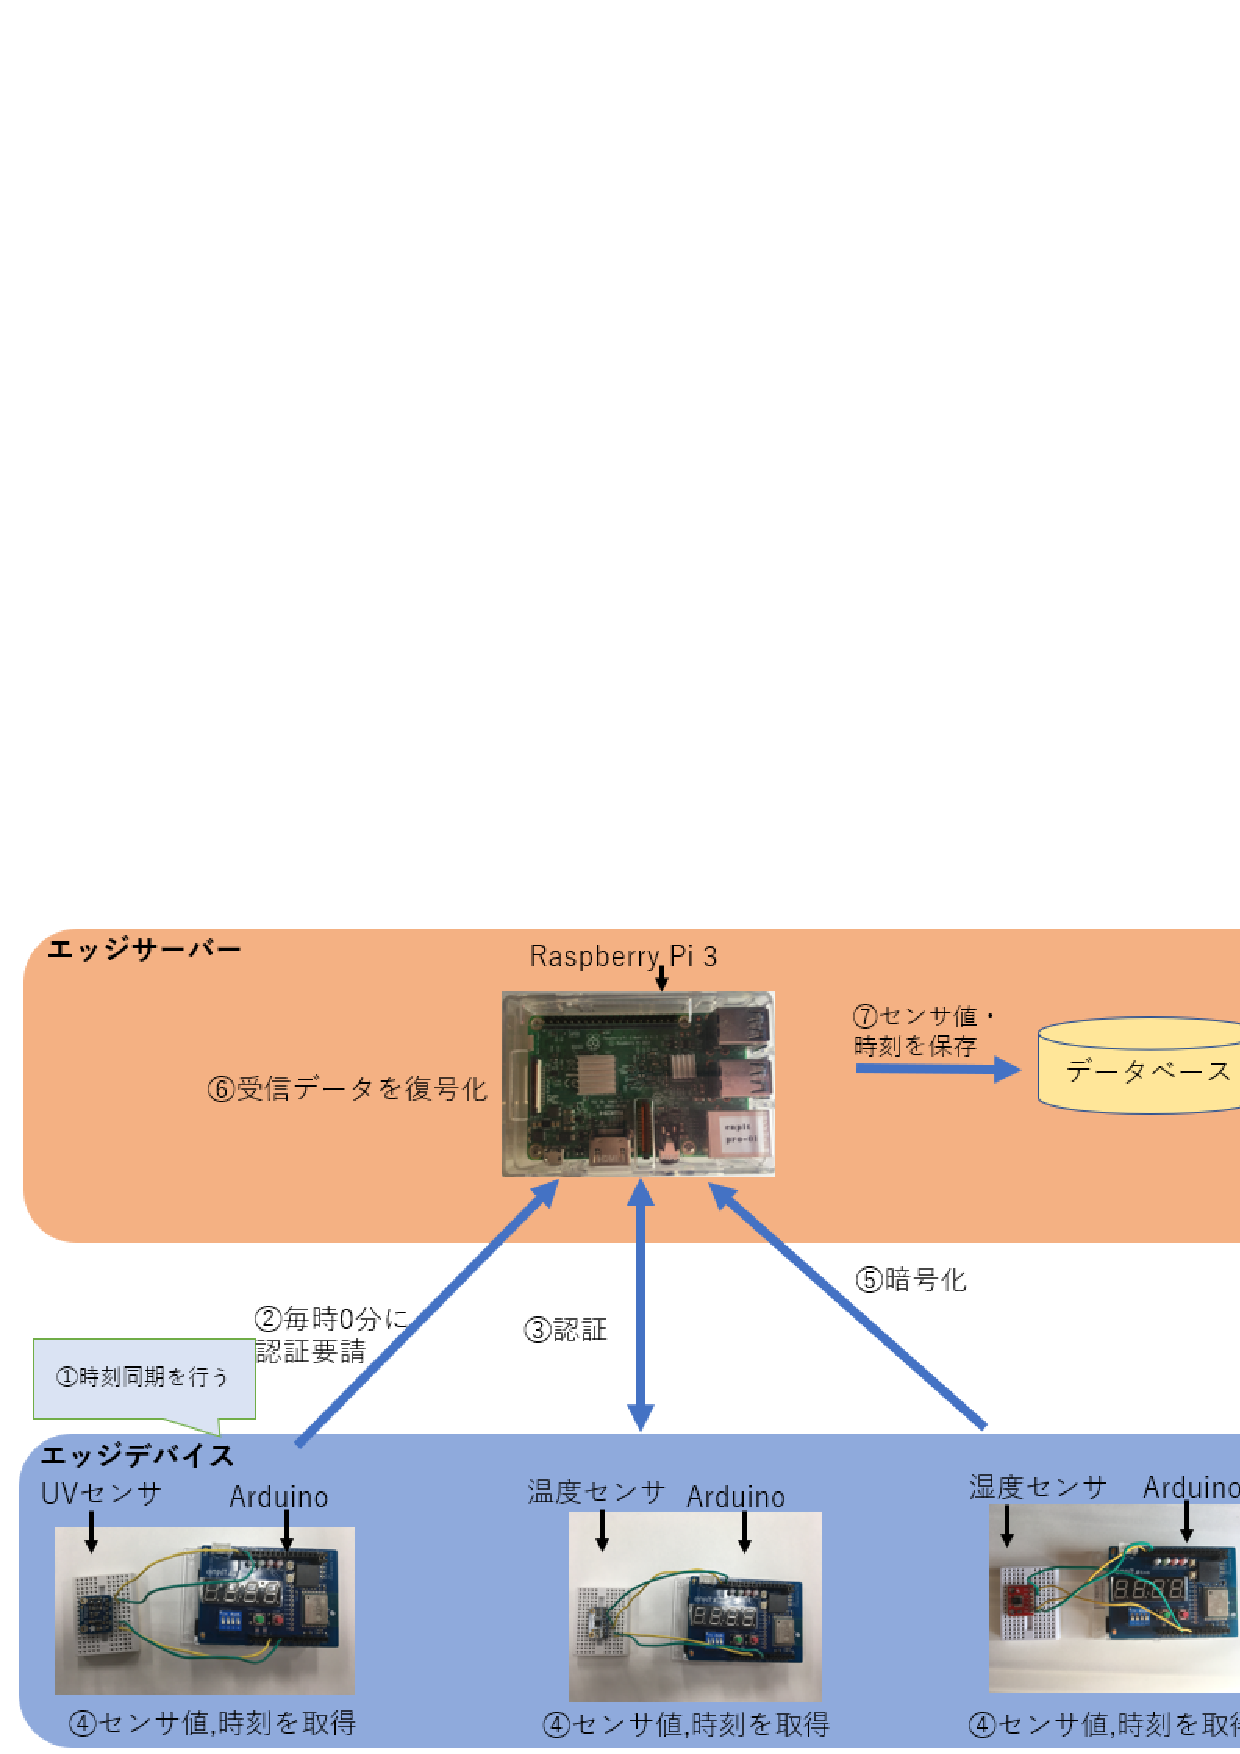
\includegraphics[height=80mm]{gaiyo.png}
	\caption{SAS-L2を利用したセキュアな組込みシステムの概要図}
\label{fig:gaiyo}
\end{center}
\end{figure}

Raspberry Piをエッジサーバーとし,3台のArduinoをエッジデバイスとして利用する.
図\ref{fig:gaiyo}のように,エッジデバイスにはそれぞれ,UVセンサ,温度センサ,湿度センサを接続している.
データベースには,エッジデバイスから収集したデータを保存する.
以降,エッジサーバーをサーバー,エッジデバイスをユーザーと定義する.
図\ref{fig:gaiyo}に沿って,SAS-L2を利用したセキュアな組込みシステムの時刻同期,センシングデータ取得,認証,および暗号化通信の処理の流れを説明する.

\begin{enumerate}
	\item ユーザーを起動し,時刻同期を行う.
	\item ユーザーはサーバーに対して,指定した時刻に認証要請を行う.
	\item サーバーは認証要請を受信し,認証要請を送信したユーザーとのSAS-L2認証を行う.
	\item ユーザーは認証完了後,接続されたセンサからセンシングデータ(センサ値)と,
    センシングデータを取得した日時を取得する.
	\item ユーザーは処理4で取得したデータを暗号化しサーバーへ送信する.
	\item サーバーはユーザーから受信したデータを復号し,センシングデータと日時を取得する.
    \item サーバーは取得した,センシングデータと日時をデータベースに保存する.
    \item 処理4から処理7を10回繰り返す.
    \item 処理2から処理8を繰り返す.
\end{enumerate} 

以上のように,指定した時刻になると認証1回,暗号化通信10回を行うシステムとなる.

\section{要件定義}
SAS-L2を利用したセキュアな組込みシステムの要件定義を述べる.
要件定義には,機能要件と非機能要件がある.
機能要件は,システムで実現すべき機能であり,クライアントから求められる機能のことである.
非機能要件は,機能要件以外の要件であり,主に性能やセキュリティ,環境,制約を指す.
\subsubsection{機能要件}
\begin{enumerate}
	\item 指定した時刻にユーザ―からサーバーにコネクションして認証要請を送信する.
	\item サーバーとユーザー間でSAS-L2による認証を行う.
    \item 認証が成功した場合,サーバーとユーザー間でSAS-L2に基づいた暗号化通信を行う.
    \item 認証が失敗した場合,コネクションを切断してシステム概要で述べた処理1からやり直す.
	\item サーバーは受信データを復号してセンシングデータと日時をデータベースへ保存する.
    \item 暗号化通信終了後,サーバーはコネクションを切断し,ユーザーからの認証要請待ち状態となる.
\end{enumerate} 

\subsubsection{非機能要件}
\begin{enumerate}
    \item 複数のユーザーは同時刻に認証要請を送信するので,一台の認証が終了するまで,その他のユーザーは待機状態になる.
    \item サーバーは認証結果をユーザーに送信する.
    \item サーバーとユーザーは認証結果を表示する.
    \item ユーザーは,シリアルモニタに取得したセンシングデータとセンシングデータの取得日時を表示する.
    \item ユーザーは起動後,1度時刻同期を行う.
    \item サーバーは暗号化通信の際,5秒以上データを受信できなければ,コネクションを切断し,認証要請受信の待機状態となる.
	\item 指定した時刻毎に3つのユーザーとの通信を10秒以内に終わらせる.
    \item サーバーはセンシングデータと取得日時を保存する際に,ユーザーごとのテーブルに分けて保存する.
    \item 1度の認証につき,10回の暗号化通信を行う.
	\item ユーザーで,何らかのエラーが発生した場合,赤LEDを点滅させる.
\end{enumerate} 


\chapter{SAS-L2を用いたセキュアな組込みシステムの設計}
%第5章
本章では、本システムに対する評価・考察を行い、今後の課題や将来性についても述べる。

まず3.1節に挙げた、本システムが果たすべき2つの大きな役割に対して評価する。3.1節において、本システムが果たすべき役割について、「感染症予防対策のルールを守ってもらうよう働きかける役割」、「感染症予防対策の基準を定める役割」の2つを挙げた。感染症予防対策のルールを守ってもらうよう働きかける役割については、室内環境に応じた換気要請の発出や、感染リスクのレベルの通知によって、換気や人数調整といった具体的なアクションを促すことが実現できていると考えられる。感染症予防対策の基準を定める役割については、利用者が感染症予防のためにとるべき、換気と部屋に滞在する人数の調整というアクションについて、感染症予防の観点から、部屋を安全な状態に保つため、具体的にその基準を定めることで、利用者自身が感染症予防のためにとるべきアクションを明確にすることが実現できていると考えられる。

また本システムでは、センサデバイスで取得したデータを随時データベースに記録しているほか、室内の滞在人数や警戒レベル、感染リスクといったデータも、センサデバイスからのデータ更新に伴って導き出されていることから、必要に応じてデータを保管しておくことで、システム外部で様々なデータの相関を調べることもできる。そのため、感染症予防対策の基準を定める役割に関しては、応用の余地があると考えられ、例えば以下のような応用の仕方が考えられる。

本システムでは、分析に活かせる多くのデータを導き出せるが、中でも設計の段階から分析に役立てられるデータとして着目していたのは、警戒レベルと感染リスクのデータである。既に述べたように、室内にある程度の人数が滞在していないと警戒レベルの導出は行われない。そのため警戒レベルの推移のデータは、その部屋が警戒レベルを導出できる条件下で利用されているとき、どの程度二酸化炭素濃度が高まりやすいかを確認でき、運用ルール改定の基準にできる。また、警戒レベルと感染リスクのデータをシステム内部で分析し、本システムでは固定的である、二酸化炭素濃度と警戒レベル、警戒レベルと滞在可能人数の関係を、部屋の警戒レベルと感染リスクの変動の仕方に応じて流動的に変化させると、よりその部屋にあった感染症予防対策を講じることが可能になると考えられる。

感染リスクのデータは、換気状況など、部屋の運用の仕方が適切であるかどうかを示しているため、部屋が感染症予防対策上、危険な状態で使用されていないかを確認できる。そのため学校やオフィス、公共施設などでの利用のケースを想定すると、時間帯ごとの感染症予防対策への取り組みの徹底度合いが、エビデンスとして残されることから、管理者側からの適切な指導が行えるほか、各部屋の責任者となる者が、感染症予防対策に、より注意して取り組むことができると考える。

本システムの設計時の着想では、利用環境ごとに異なる、床面積の広さ・空間の広さ、換気のしやすさや窓の位置と数、換気設備の有無、部屋利用者の活動の仕方などに柔軟に対応し、利用環境に合わせた感染症予防対策の基準を定め、利用者に感染症予防対策のルールを守ってもらうよう働きかけられることが本システムの特徴であった。実際に、本システムは4.2節の総合テストでの検証のように、様々なシナリオにあった感染症予防の働きかけが可能となることが考えられる。しかしながら、本システムでの感染症予防対策の基準の決め方では、換気のしやすさや、部屋の床面積の広さのわりに、ものが多く置かれているなどの理由から実際の空間が狭いというような部屋の特性が、そのまま二酸化炭素濃度の上昇の仕方に反映されることを前提としている部分があり、柔軟性に欠けていると考える。理想的な環境における本システムの実用性は確認されたものの、部屋ごとの特性を加味した感染症予防対策の基準を、実際の利用環境において適切に定めるためには、本システムでの室内環境の分析の仕方よりも複雑に、室内環境を分析する必要があるとも考えられ、部屋の特性自体をシステムの分析機能によって導き出すことができると、現在のシステムと比較し、よりその部屋の特性に適合した感染症予防対策の基準の設定を行うことができるため、更なる研究と改良の余地が大いに残されていると考える。




\chapter{検証}
%あとがき
本研究ではセンシング技術、物体検出技術、および複数デバイス間の無線通信という3つの技術とデータ分析の組み合わせによって、感染症予防という、研究・実用化が活発に進められる分野において新たな価値を生み出すことができた。感染症予防に関しては、既に様々な分野で研究・開発がなされているものと思われるが、今回私たちが開発したシステムも、感染症予防の取組を援用するシステムとして貢献できると考える。

また今回の研究では、感染症予防のために活用できるシステムの社会的な必要性が高まり、多くの企業や研究機関により研究・開発が進められている状況下で、感染症予防のために用いるシステムとして、3 密回避に役立てられるという、新型コロナウイルスの世界的な流行以前にはなかった新しい価値を持たせることも、1つの目標として定められた。本研究において、私たちの考える感染症予防のサポートシステムの基本形を提案することができた。今後さらなる研究が進められれば、より高いリアルタイム性と精度を併せ持つモニタリングと、感染症予防対策基準の設定機能における更なる柔軟性を実現でき、より利用しやすいものへと改良が進められることから、拡張性のある研究であると考える。


\chapter{あとがき}
%あとがき

本研究の研究背景としてIoTデバイスに対するセキュリティ対策として認証・暗号化通信を行うことが挙げられるが,処理性能の低いIoTデバイスでは従来法の暗号方式での実装が困難である.
そこで,本研究ではワンタイムパスワード認証方式SAS-L2をIoTセンシングデバイス
に実装することで,デバイス間の認証およびセンシングデータの暗号化通信方法を実現することを目標に開発を行った.
SAS-L2認証方式を導入したIoTシステムの設計はUMLのユースケース図,クラス図,シーケンス図などを用いて行い,
その設計に基づきチームで分担し開発を行った.実装完了後は,V字開発モデルに従って,単体テスト,結合テスト,総合テストの順でテストを行った.
検証結果から,SAS-L2認証方式をセンシングデバイスに実装し,
デバイス間の認証とSAS-L2に基づいたデータ通信の暗号化ができたことが分かる.
また,センシングデータの暗号化では,排他的論理演算2回で済むため,処理能力の低いセンシングデバイスにおいてリアルタイムでの暗号化通信を実現することができる.
そして,問題点と課題として,センシングデバイスに初期認証情報や初期秘匿情報が書き込まれていない場合,
初期情報を取得する際の安全な方法の確立について,そして,認証情報と秘匿情報を不揮発性メモリに書き込む場合,
不揮発性メモリの書き込み回数を考慮して認証回数の決定をしなくてはならないという点が挙げられる.
それらを改善することで,本システムでの処理性能の低いセンシングデバイスに認証方式と暗号化通信を導入することによる,さらなるセキュリティ強化に繋がると考える.


%謝辞
\newpage
\addcontentsline{toc}{chapter}{\protect\numberline{謝辞}{}}
\chapter*{謝辞}
%--ここから謝辞--

本研究を進めるにあたり,懇篤な御指導,御鞭撻を賜わりました本学高橋寛教授に深く御礼申し上げます.

本論文の作成に関し,詳細なるご検討,貴重な御教示を頂きました本学高橋寛教授ならびに甲斐博准教授,王森レイ講師に深く御礼申し上げます.

また,審査頂いた本学高橋寛教授,樋上喜信教授,井門俊講師に深く御礼申し上げます.

最後に,多大な御協力と貴重な御助言を頂いた本学工学部情報工学科情報システム工学講座高橋研究室の諸氏に厚く御礼申し上げます.

%--ここまで謝辞--

%参考文献
\begin{thebibliography}{99}
%ここから参考文献

\bibitem{maegaki}
IPA独立行政法人情報処理推進機構技術本部セキュリティセンター.“IPAテクニカルウォッチ「自動車の情報セキュリティ」に関するレポート".IPA独立行政法人情報処理推進機構.
\url{https://www.ipa.go.jp/files/000009384.pdf},
(参照2022-01-05)
\bibitem{AES}
斉藤貴之.“3分でわかるAES".日経クロステック.
\url{https://xtech.nikkei.com/atcl/nxt/keyword/18/00002/030800119/},
(参照2022-01-05)
\bibitem{banamu}
“最強の暗号?バーナム暗号".kakke18's blog.2019-02-22.
\url{https://kakke18.hatenablog.com/entry/2019/02/22/193223},
(参照2022-01-05)
\bibitem{tcp/udp}
竹下隆史,村山公保,荒井透,苅田幸雄.マスタリングTCP/IP入門編第5版.オーム社.2019.
\bibitem{sas-l}
清水明宏.SAS-L ワンタイムパスワード認証方式について.preprint.2020.
\bibitem{vmodel}
水野忠則,中篠直也,井上雅裕,山田圀裕.未来へつなぐデジタルシリーズ20 組込システム.共立出版.2017.
\bibitem{uml}
永和システムマネジメント.“UML超入門".オブラブ.
\url{http://objectclub.jp/technicaldoc/uml/umlintro},
(参照2022-01-05)
%ここまで参考文献

\end{thebibliography}
\end{document}



